\documentclass{article}
\usepackage[letterpaper, margin=0.95in]{geometry}
\usepackage[T1]{fontenc}
\usepackage{titleps}
\usepackage{parskip}
\usepackage{booktabs}
\usepackage{graphicx}
\usepackage{xcolor}
\usepackage{microtype}
\usepackage[hidelinks]{hyperref}

\newpagestyle{ruled}
{\sethead{CMU 16-831}{Intro to Robot Learning}{Fall 2026}\headrule
  \setfoot{}{}{}}
\pagestyle{ruled}
\renewcommand\makeheadrule{\color{black}\rule[-.75\baselineskip]{\linewidth}{0.4pt}}

\begin{document}

\begin{center}
    {\Large Assignment 1: Imitation Learning} \\
    \vspace{.25cm}
    \textbf{Andrew ID:} \texttt{mlin4} \\
    \textbf{Collaborators:} \texttt{None}
\end{center}

% \textit{Generative AI tools such as ChatGPT are viewed as collaborators in this course, acknowledge accordingly.}

\section{Behavioral Cloning (10 pt)}

\subsection{Part 2 (1.5 pt)}
\begin{table}[!h]
  \centering
  \caption{Mean and standard deviation of expert return over two trajectories, for each environment.}
  \begin{tabular}{cccccc}
    \toprule
    Metric/Env & Ant-v2 & Humanoid-v2 & Walker2d-v2 & Hopper-v2 & HalfCheetah-v2 \\
    \midrule
    Mean  & 4713.65	& 10344.52  & 5566.85   & 3772.67 & 4205.78 \\
    Std.  & 12.20   & 20.98     & 9.24	    & 1.95	  & 83.04 \\
    \bottomrule
  \end{tabular}
  \label{tab:p2}
\end{table}

\subsection{Part 3 (5 pt)}
\begin{table}[htbp]
  \centering
  \caption{BC vs.\ expert return. List the environment you chose and the hyperparameters (network size, amount of data, training iterations, \texttt{eval\_batch\_size}, etc.) here.}
  Hyperparameters: \texttt{n\_layers}~$=3$, \texttt{size}~$=128$, \texttt{learning\_rate}~$=10^{-3}$, \texttt{num\_agent\_train\_steps\_per\_iter}~$=10{,}000$, \texttt{train\_batch\_size}~$=100$, \texttt{eval\_batch\_size}~$=5000$, \texttt{n\_iter}~$=1$, seed~1. Training data: 2 expert trajectories (2000 transitions).
  \begin{tabular}{ccccc}
    \toprule
    Env   & \multicolumn{2}{c}{Ant-v2} & \multicolumn{2}{c}{Humanoid-v2} \\
    \midrule
    Metric & Mean  & Std.  & Mean  & Std. \\
    Expert & 4713.65 & 12.20 & 10344.52 & 20.98 \\
    BC    & 4732.75 & 100.06 & 288.89 & 21.48 \\
    \bottomrule
  \end{tabular}
  \label{tab:p3}
\end{table}

\subsection{Part 4 (3 pt)}
\begin{figure}[!h]
  \centering
  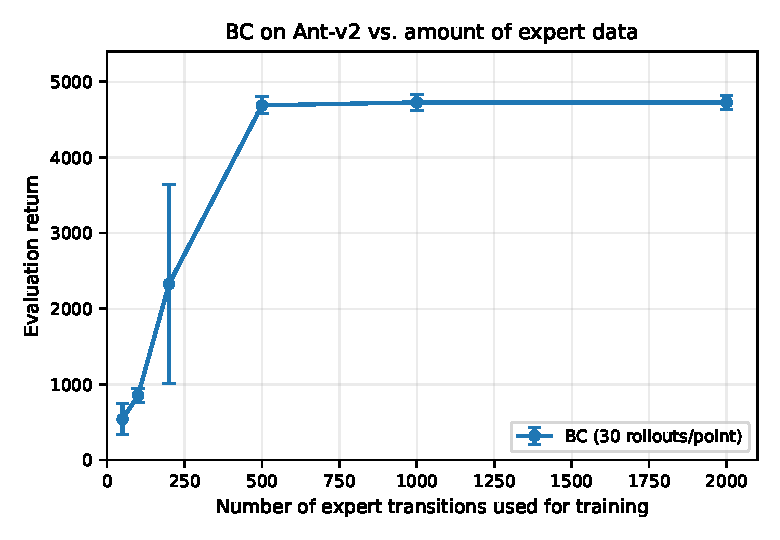
\includegraphics[width=0.5\columnwidth]{p4_plot.pdf}
  \caption{BC on Ant-v2 vs.\ the number of expert transitions used for training, subsampled from the 2 provided trajectories. Network (3$\times$128), \texttt{lr}~$=10^{-3}$ and 10{,}000 gradient steps are held fixed; each point is the mean over 30 rollouts (3 seeds $\times$ \texttt{eval\_batch\_size}~$=10{,}000$) and the error bars are the std across those rollouts. I expected BC to get gradually worse as I removed data, but it stays at expert level down to 500 transitions and then falls off fast, so my hypothesis was wrong.}
  \label{fig:p4}
\end{figure}

\subsection{Part 5 (0.5 pt)}
\textit{Learning Fine-Grained Bimanual Manipulation with Low-Cost Hardware} (2023) introduces ACT (Action Chunking with Transformers) which utilizes behavior cloning. The behaviors are dexterous manipulation skills such as slotting a battery and opening a condiment cup, and the expert data is human teleoperation of a pair of leader arms. The main risk from this homework, compounding error under distribution shift, applies directly since ACT is trained with no DAgger-style interactive relabeling to correct for policy drifting. The paper tries to mitigate this proble by predicting a chunk of $k$ future actions rather than one step at a time, which shortens the effective decision horizon. This reduces how quickly errors accumulates in their experiments.


\newpage
\section{DAgger (5 pt)}

\subsection{Part 2 (5 pt)}
\begin{figure}[!h]
  \centering
  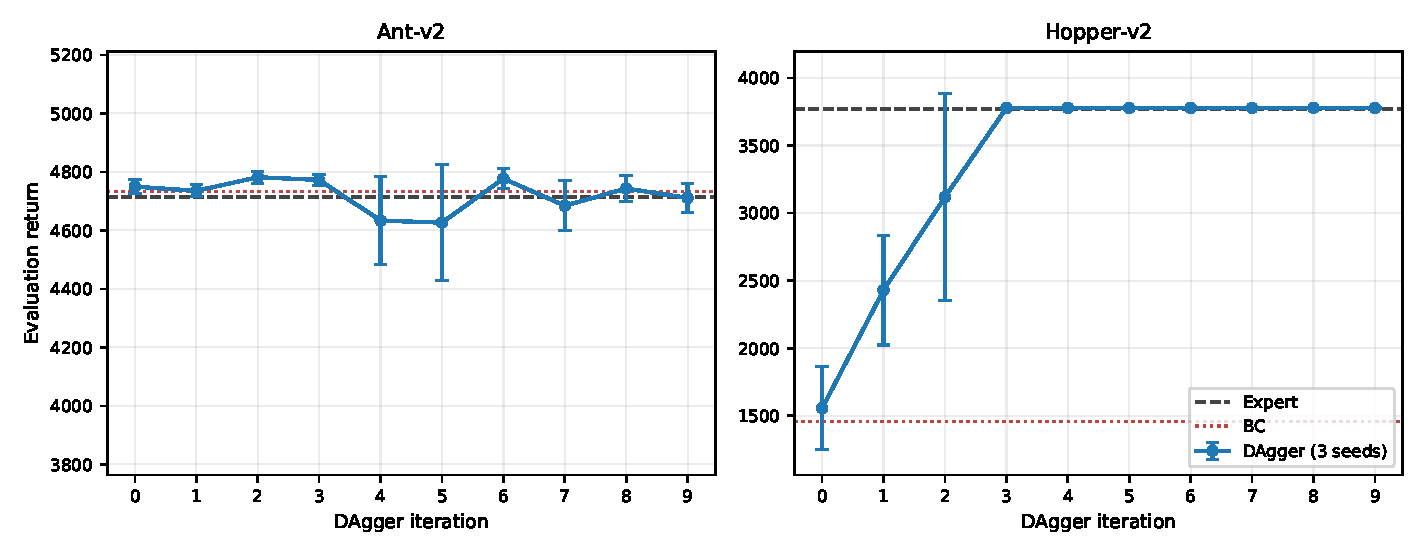
\includegraphics[width=\columnwidth]{dagger_plot.pdf}
  \caption{DAgger learning curves (mean return vs.\ iteration, with error bars). Ant-v2 on the left and Hopper-v2 on the right. Dashed $=$ expert, dotted $=$ BC. Policy: 3$\times$128 MLP, \texttt{lr}~$=10^{-3}$, 10{,}000 gradient steps/iteration, starting from 2 expert trajectories and adding 1000 relabeled transitions per iteration.}
  \label{fig:p5}
\end{figure}


\end{document}
